\section*{Goldponsor und Aussteller}
\begin{flushright}
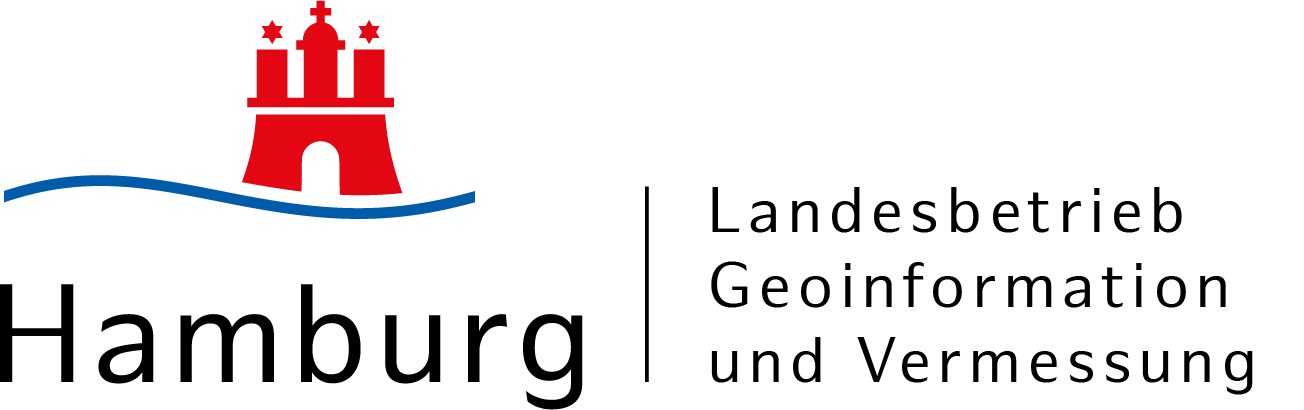
\includegraphics[width=1.0\textwidth]{102_LGV.png }
\end{flushright}
\noindent
Der {\bfseries Landesbetrieb Geoinformation und Vermessung (LGV)} ist der zukunftsgestaltende und innovative Dienstleister, wenn es um die Erhebung, Pflege und Bereitstellung von (Geo-)Daten geht. Zu seinem Angebotsportfolio gehören IT-basierte urbane (Geo-)Anwendungen genauso, wie 3D-Darstellungen, Datenanalysen, alle vermessungsrelevanten Aufgaben sowie Immobilienbewertungen.

\noindent
Aufgrund seiner langjährigen Erfahrung in der Geodäsie und Geoinformation ist der LGV nicht nur in Hamburg, sondern auch bundesweit Impulsgeber und technologischer Vorreiter für die digitale Vernetzung und Online-Darstellung von (Geo-)Daten.

\noindent
Als Teil der Hamburger Behörde für Stadtentwicklung und Wohnen agiert der LGV seit 2003 eigenständig. Circa 370 Beschäftigte kümmern sich in Hamburg-Wilhelmsburg um die städtischen Anforderungen seitens der Bürgerinnen und Bürger, Verwaltungen und Wirtschaft. Der LGV unterstützt den Senat bei der Umsetzung seiner Strategie „Digitale Stadt“.

